\documentclass[12pt]{article}
\usepackage[latin1]{inputenc}
\usepackage{html,makeidx}
\usepackage{enumerate}
\usepackage{amsmath}
\usepackage{graphicx}

\title{The KrdWrd Add-on}
\author{Maria Cieschinger, Kilian Klimek, Egon Stemle}
\begin{document}
\maketitle

\section{Introduction}


"The availability of large text corpora has changed the scientific approach to language in linguistics and cognitive science" [M\&S].
Today, the by far richest source for authentic natural language data is the World Wide Web, and making it useful as a data source for scientific research is imperative.

Web pages, however, can not be used for computational linguistic processing without filtering:
They contain code for processing by the Web browser, there are menus, headers footers, form fields, teasers, out-links, spam-text -- all of which needs to be stripped.

The dimension of this task calls for an automated solution, the broadness of the problem for machine learning based approaches.
Part of the KrdWrd project deals with the development of appropriate methods, but they require hand-annotated pages for training.

The \textit{KrdWrd Add-on} aims at making this kind of tagging of Web pages possible.
For users, we provide accurate Web page presentation and annotation utilities in a typical browsing environment, while preserving the original document and all the additional information contained therein.


\section{Getting Started}
In this section, we will give you information about how to use the tool. If you have not installed it yet, go to \htmladdnormallink{krdwrd.org}{https://krdwrd.org/trac/wiki/AddOn} and get it. Of course, you will need \htmladdnormallink{Firefox}{http://www.mozilla.com}, too. \\

\begin{itemize}
\item Since the add-on depends on a special proxy server to connect to the Internet - you can only grab and submit Web pages from the KrdWrd corpora - it may be a good idea to create a separate profile just for working with the add-on. If you want to create a profile but have no idea how to do that, have a look \htmladdnormallink{here}{http://kb.mozillazine.org/Profile_Manager}. \\
\item When grabbing a page for the first time, or selecting a corpus for the first time you will be asked to authenticate for the \htmladdnormallink{krdwrd Off-Line Proxy}{https://krdwrd.org/trac/wiki/WebProxy}. The username and password in the dialog box are already filled in and it is save to leave the "Use Password Manager to remember this password" checked. \\

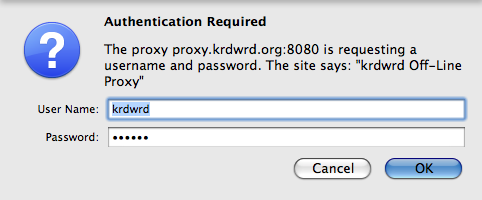
\includegraphics[width=0.6\textwidth]{images/prxylogin.png}
\medskip

\item The proxy server will deny all requests that are not part of the normal add-on operation. If you ever see something like \\

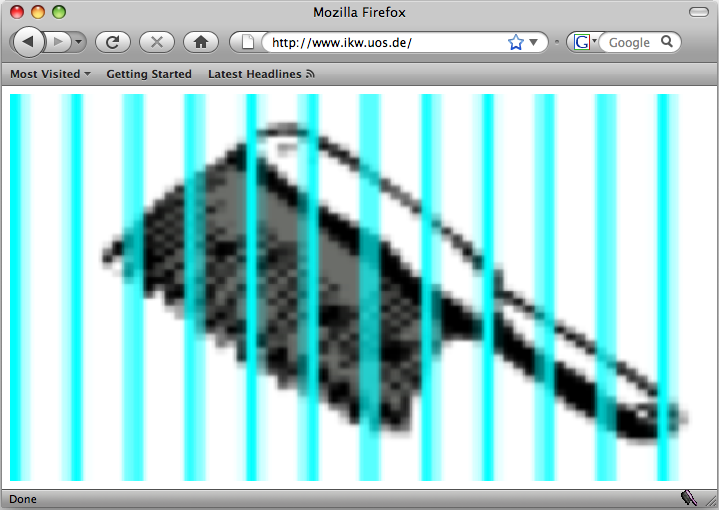
\includegraphics[width=0.6\textwidth]{images/blocked.png}
\medskip

it is most likely because you tried to surf the Web with the wrong Firefox profile. \\

\item You will be asked for authentication a second time. This authentication is for the KrdWrd Web site and requires your \emph{RZ Account}\footnote{This is the same login as for \emph{Stud.IP} and \emph{WebMail}; in case you want to "Use Password Manger" please also "Use a master password" to protect your sensitive information.} \\

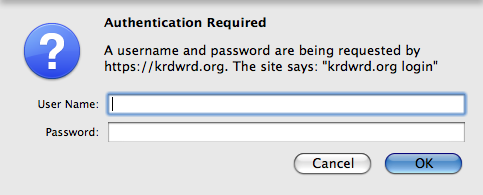
\includegraphics[width=0.6\textwidth]{images/stlogin.png}
\medskip

\item When you request a page from the corpus for the first time, Firefox will popup a security warning. The warning says \emph{"you have requested an encrypted page that contains some unencrypted data"}. The warning is issued because the corpus page are issued unencrypted. Your login credentials are never send to the server unencrypted, there is no reason not to ignore this warning. \\

\end{itemize}


\subsection{First Steps}

\begin{itemize}
	\item {\large \textbf{How to Use the Mouse}}\\
When moving the mouse over a Web page, you will notice that certain areas are highlighted in pink. These are the blocks of text that you can tag. Sometimes the pink areas are fairly small (single words or lines of text), sometimes they are pretty large (whole paragraphs, or even whole pages). Thus it makes sense to move the mouse around a little before you actually start tagging because sometimes you want to tag big areas as, say, 'bad', and it saves you a lot of time if you do not have to tag every single line or paragraph. As a rule of thumb, it often makes sense to tag \emph{everything} in red ('bad'), from top to bottom, and only then start tagging smaller pieces in yellow or green ('uncertain' or 'good', respectively) (see also \textbf{\hyperref{Examples}{Examples, described on page~}{}{Examples}, \hyperref{Tips \& Tricks}{Tips \& Tricks, page ~}{}{TnT}}).\\ \\


	\item {\large \textbf{How to Choose the Tag}}\\

This section deals with assigning tags. If you want information on how to choose the \emph{right} tag to assign, go to the \hyperref{Annotation Guidlines}{Annotation Guidlines on page ~}{}{Annotation}. \\

For tagging a pink-highlighted section as 'good', 'bad', or 'uncertain', you have two options: You can use (1) keyboard shortcuts (hotkeys) or you can use (2) the context menu (rightclick).\\
\begin{enumerate}
	\item Keyboard Shortcuts
		\begin{itemize}
			\item \emph{bad}: ctrl+alt+1
			\item \emph{uncertain}: ctrl+alt+2
			\item \emph{good}: ctrl+alt+3
			\item \emph{clear annotation}: ctrl+alt+4
		\end{itemize}
	\item Context Menu
		\begin{itemize}
			\item Rightclick when you are over the section you want to tag, then choose KrdWrd, and then the tag you want to assign. 
				\smallskip
				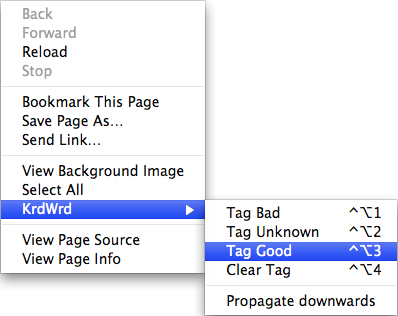
\includegraphics[width=0.5\textwidth]{images/ctxmenu.png}
				\medskip
			\item Using the context menu is not recommended, however. It is much more time-consuming to navigate the menu than to use the keyboard shortcuts.
			\item Note also that if the mouse cursor leaves the menu area, a possibly different part of the page will be highlighted for tagging (namely the part that is now 'under' your mouse).
		\end{itemize}
\end{enumerate}

	\item {\large \textbf{Cookies and Certificates}}\\
When some of the pages are being loaded, your Web browser will ask you whether you want to accept cookies (of course, depending on your browser settings: If you use a separate profile for the KrdWrd add-on, just allow all cookies, see \hyperref{Tips \& Tricks}{Tips \& Tricks, page ~}{}{TnT}). Actually, you \emph{do not} have to accept any cookies; however, nothing bad will happen if you do accept them.
\end{itemize}

\subsection{The Statusbar Menu}

This section describes the status bar menu, depicted below. \\

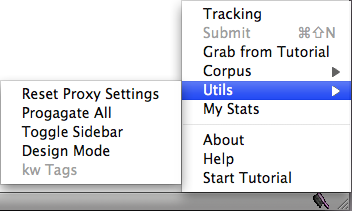
\includegraphics[width=0.6\textwidth]{images/stsbrmenu.png}
\medskip

\begin{itemize}
	\item {\large \textbf{Tracking}}\\
Here you can turn on or off whether sections of the Web page you are currently viewing are highlighted in pink. Usually there is no need to disable tracking. However, in some rare cases, this might help you to get a better view on a page before tagging it. \\
	\item {\large \textbf{Submit}}\\
When you are done tagging a page, i.e.~when everything on the page is green, red, or yellow, you can submit the page with this menu option - and the next page will load automatically. For your convenience, you can also use the keyboard shortcut \emph{options+shift+N}. \\

	\item {\large \textbf{Grab Page}}\\
Clicking here loads a new, un-annotated page. Once you annotated the whole corpus, you will be redirected to your personal statistics page. \\ \\
	\item {\large \textbf{Corpus}}\\
Here you can select one of the (predefined) available corpora. But you should stick to the Canola corpus for now.\\ \\
	\item {\large \textbf{Utils}}\\
The options in this menu make your life easier when tagging pages. \\
	\begin{itemize}
		\item {\large \textbf{Propagate}}\\
Here you can explicitly propagate a given tag down to all sibling nodes. This is helpful when you have a large portion that should be tagged red but all its siblings should be tagged green. You can then tag the parent node green, propagate, and re-tag the parent node as red. This way you do not need to tag all the siblings separately. (Try this on the \hyperref{Examples}{Examples, described on page~}{}{Examples} and check the \hyperref{Tips \& Tricks}{Tips \& Tricks, page ~}{}{TnTProp}).
		\item {\large \textbf{Toggle Sidebar}}\\
Clicking here opens the sidebar. In the sidebar you can see all of the text in the current page and how it is tagged. A given tag is usually propagated down to lower nodes in the DOM tree automatically, but sometimes it may be unclear (i.e. not directly visible in the page) how a particular portion of text is tagged. In the sidebar you can easily see whether it is tagged red, green, or yellow.
		\item {\large \textbf{Design Mode}}\\
This is a debugging feature and you must not use it while tagging pages. \\
	\end{itemize}
	\item {\large \textbf{My Stats}}\\
This menu option will send you to your KrdWrd account. There you can see how many pages you have already tagged, and you can view, re-submit and delete your tagged pages. 
\end {itemize}






\section{How to Tag Pages}

\subsection{Annotation Guidelines}
\label{Annotation}
In the previous section, we described how to use the tool and how to assign tags. In the following, we give you guidelines regarding \emph{which} tag should be assigned to a particular kind of text.

\begin{itemize}
	\item Everything that is \emph{boilerplate} is tagged \textbf{red}. \emph{Boilerplate} is \ldots
	\begin{enumerate}
		\item all navigation information,
		\item copyright information,
		\item hyperlinks that are not part of the text,
		\item all kinds of headers and footers.
	\end{enumerate}
	$\rightarrow$ Generally speaking, boilerplate is everything that can be used interchangeably with any other Web page or could be left out without changing the general content of the page.
%	\end{enumerate}
	\item The following types of text are also tagged \textbf{red}:
	\begin{enumerate}
		\item incomplete sentences, or text in telegraphic style,
		\item text containing 'non-words' such as file names,
		\item off-site advertisements (i.e. advertisement from an external page),
		\item text in any other language than English,
		\item lists and enumerations of any kind.
	\end{enumerate}
	\item All captions are tagged \textbf{yellow}. And also everything that does not belong in the red or green category is tagged \textbf{yellow}.
	\item All text that is left is tagged \textbf{green}, i.e. \ldots
	\begin{enumerate}
		\item text made up of complete sentences, \textbf{even if it is in a list or enumeration},
		\item text that makes use of 'normal' words.
		\item text that is written in English.
	\end{enumerate}
\end{itemize}

Simple, isn't it? You will notice that on some pages you can only highlight very large areas, on others the choices are less restricted. If you tag an element, the tag assigned is propagated to all elements that are contained in this area. However, if you are not sure whether a specific element is entailed, just tag it too to be on the safe side (remember the \emph{sidebar option} mentioned in the previous section!).\\

In a previous section, we said that as a rule of thumb, it often makes sense to tag \emph{everything} in red ('bad'), from top to bottom, and only then to start tagging smaller pieces in yellow or green ('uncertain' or 'good', respectively). The easiest way to tag a whole page red is to tag the outermost rim of the page and tag that as 'bad'. Due to the tag propagation, the whole page is now tagged as 'bad'. If you want to make sure that this is so, check the sidebar (see above).\\

This may all be a bit confusing now. But fear not, in the next sections you will have the possibility to check whether you understood everything. \\


\subsection{Examples - Easy}
\label{Examples}

\begin{itemize}
\item \htmladdnormallink{Example 1}{https://krdwrd.org/pages/bin/view/432} \\
This is a fairly standard Web page. Advertisements and boilerplate should be easy to spot and easy to tag.\\

\includegraphics[width=0.6\textwidth]{images/432.png} \\

\item \htmladdnormallink{Example 2}{https://krdwrd.org/pages/bin/view/433} \\
This should be easy, too. \\
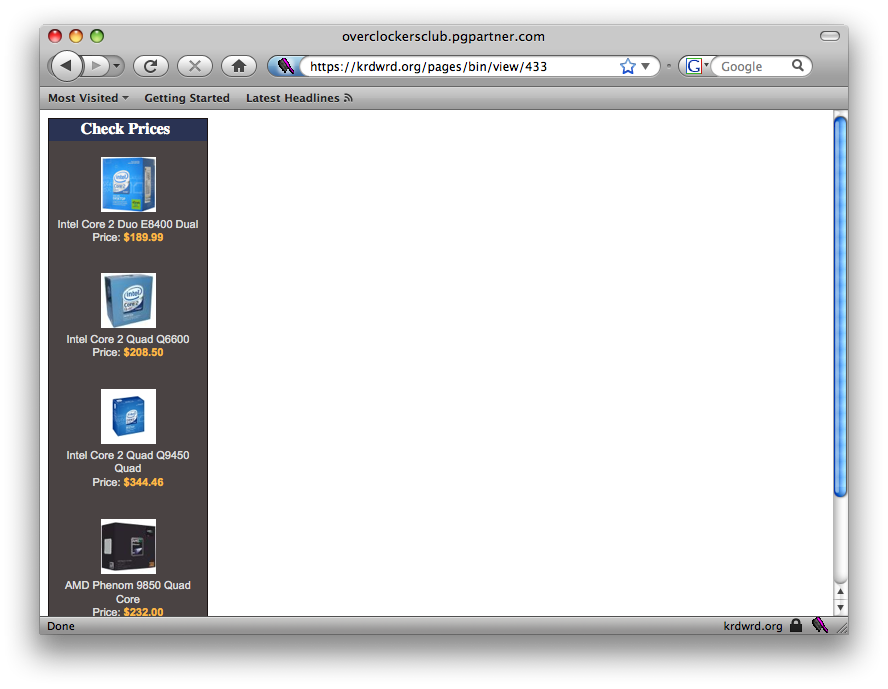
\includegraphics[width=0.6\textwidth]{images/433.png} \\

% "let it shine"
\item \htmladdnormallink{Example 3}{https://krdwrd.org/pages/bin/view/434} \\
Similar to \emph{Example 1} but you will have to invest a little more time, since the layout is not as clean. Is there something that is not 'good' in the text portion? How should you treat the headlines? What about the headlines' subtitles? \\
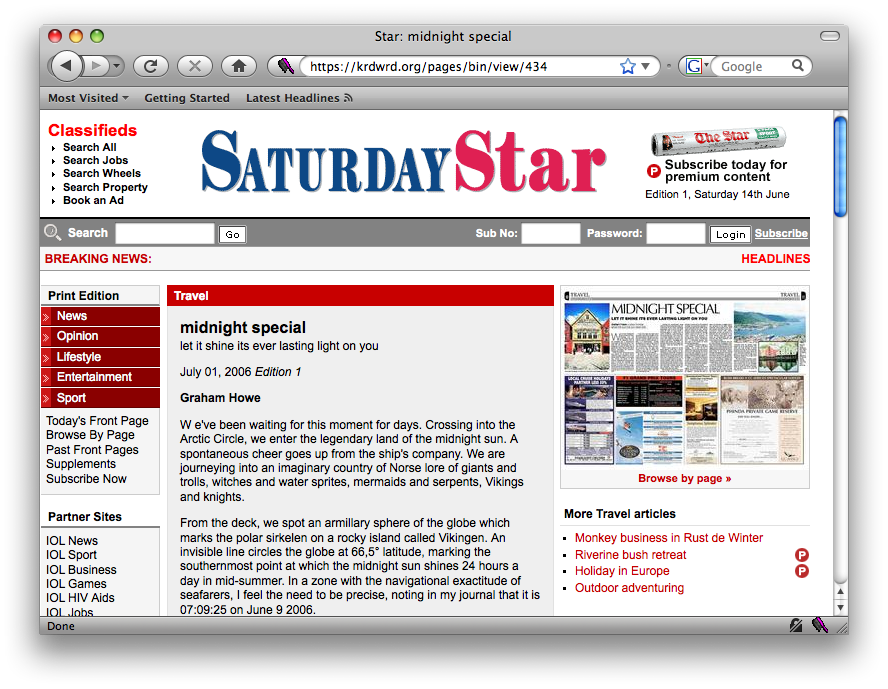
\includegraphics[width=0.6\textwidth]{images/434.png} \\

% alles rot seite
\item \htmladdnormallink{Example 4}{https://krdwrd.org/pages/bin/view/435} \\
Somehow similar to \emph{Example 2}. Why is even the text portion not 'good'? \\

\includegraphics[width=0.6\textwidth]{images/435.png} \\

\end{itemize}

\subsection{Examples - Medium}
\label{ExMedium}
\begin{itemize}
\item \htmladdnormallink{Example 5}{https://krdwrd.org/pages/bin/view/436} \\
Remember wich language you should tag (and that all text in another language is bad). How should you tag the enumerations? \\
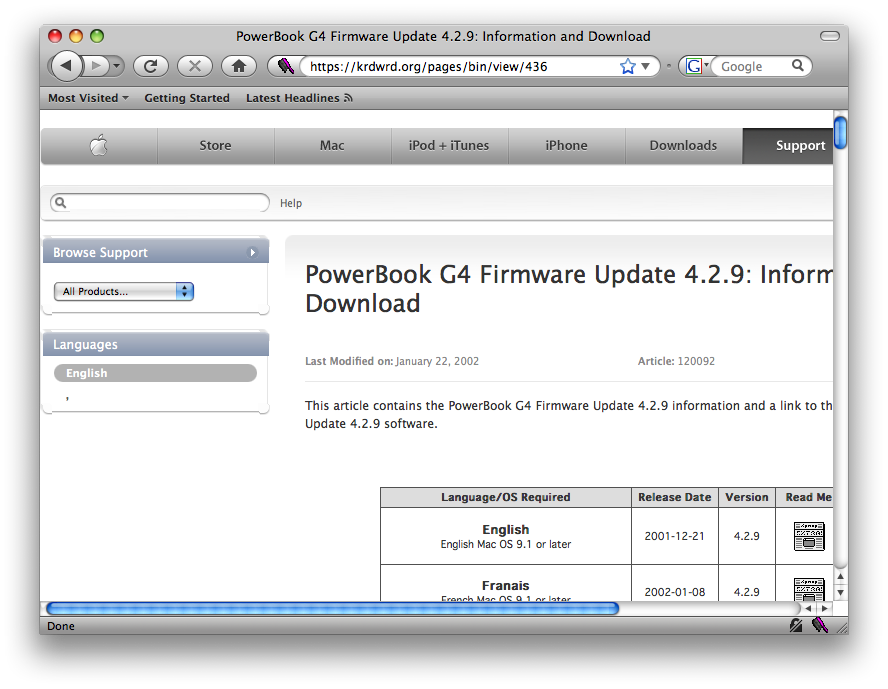
\includegraphics[width=0.6\textwidth]{images/436.png} \\

\item \htmladdnormallink{Example 6}{https://krdwrd.org/pages/bin/view/437} \\
This one is all about enumerations. \\
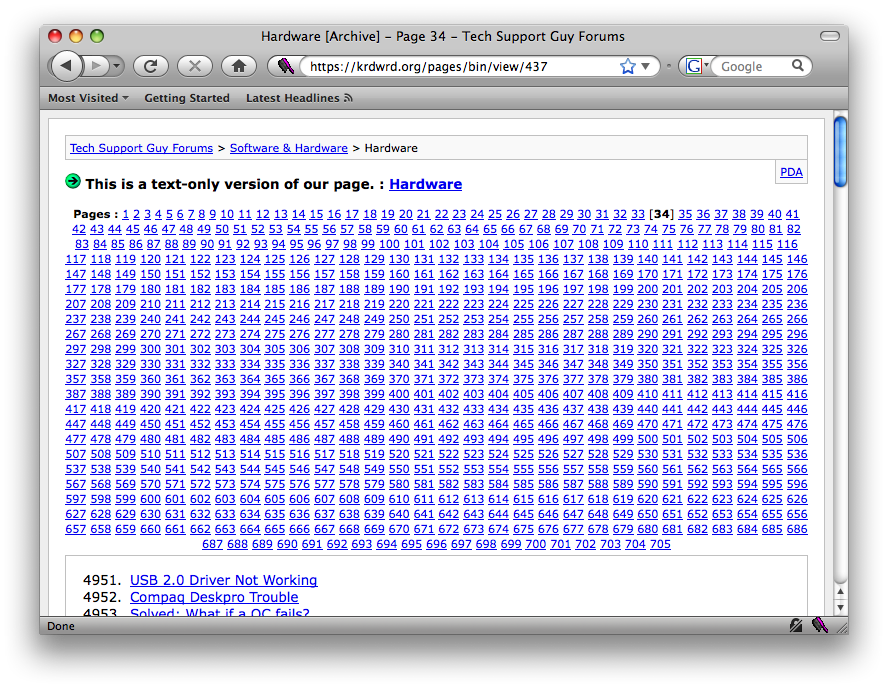
\includegraphics[width=0.6\textwidth]{images/437.png} \\

\item \htmladdnormallink{Example 7}{https://krdwrd.org/pages/bin/view/438} \\
Once you have decided how much of the text is junk, this is fairly easy. Propagate is you friend. \\
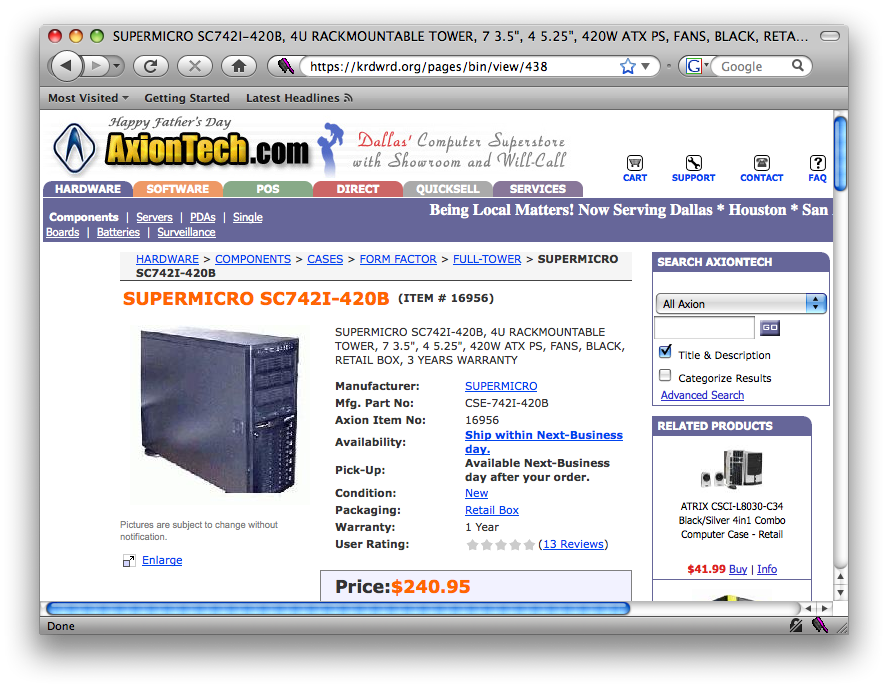
\includegraphics[width=0.6\textwidth]{images/438.png} \\

\item \htmladdnormallink{Example 8}{https://krdwrd.org/pages/bin/view/439} \\
This can be easy with the right strategy. One of the rare pages where it is easier if you don't start with tagging everything red first. \\
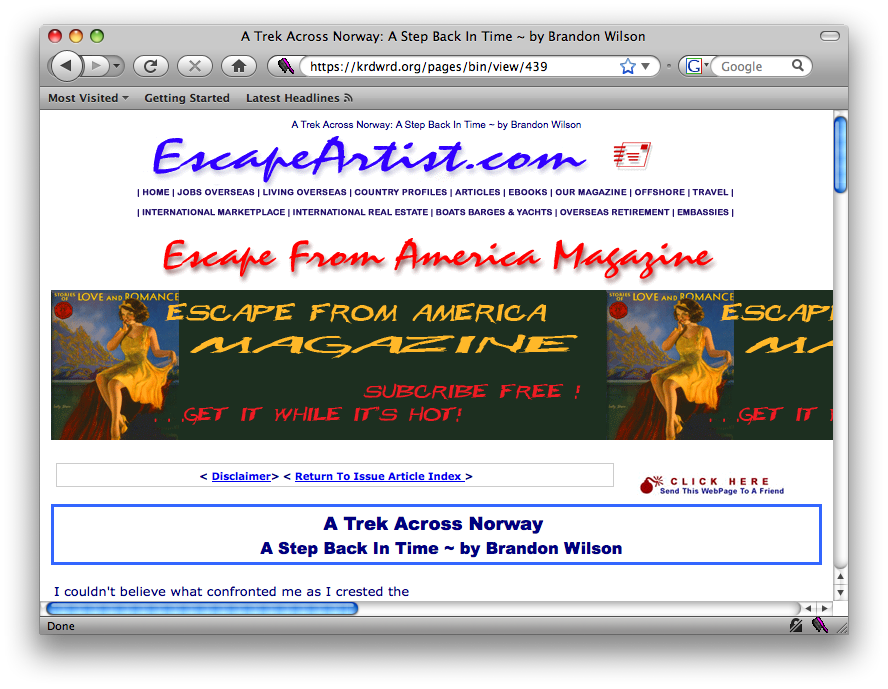
\includegraphics[width=0.6\textwidth]{images/439.png} \\

\item \htmladdnormallink{Example 9}{https://krdwrd.org/pages/bin/view/440} \\
Sometimes there are no technical difficulties. \\
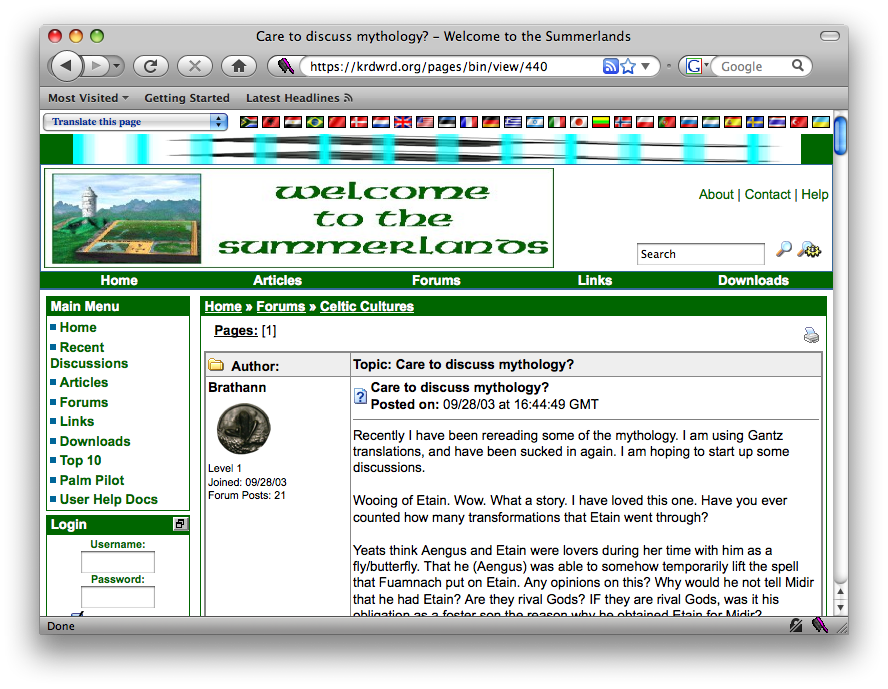
\includegraphics[width=0.6\textwidth]{images/440.png} \\

\end{itemize}

\subsection{Examples - Hard}
\begin{itemize}
% 
\item \htmladdnormallink{Example 10}{https://krdwrd.org/pages/bin/view/441}\\
By now this should be easy for you. \\
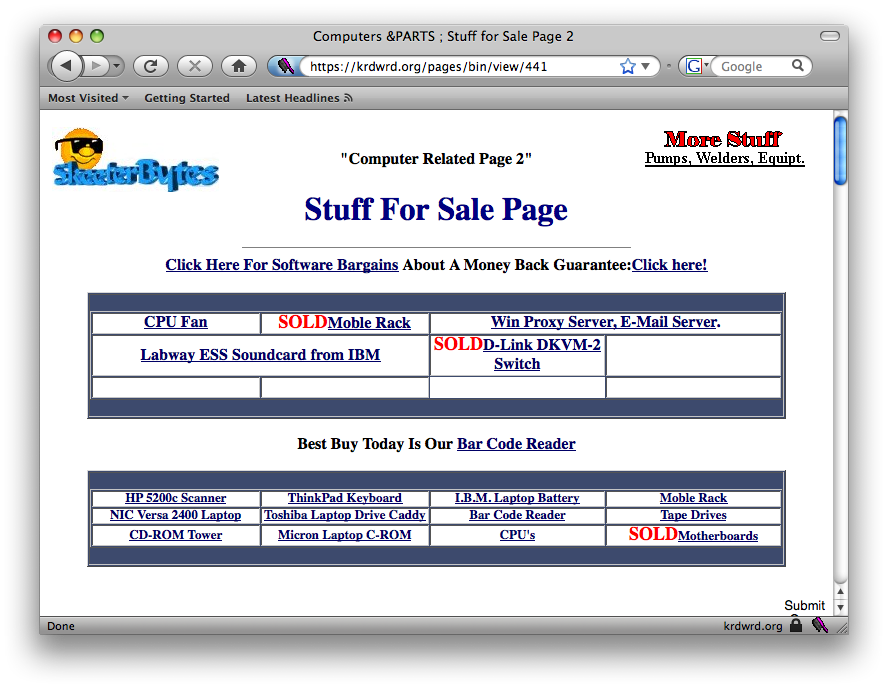
\includegraphics[width=0.6\textwidth]{images/441.png} \\

% braindamage
\item \htmladdnormallink{Example 12}{https://krdwrd.org/pages/bin/view/442} \\
This one is a bit like example 9 but with technical difficulties. You might rather want to go to your dentist. This is really as bad as it can be. If you can do this all other pages are a piece of cake. \\
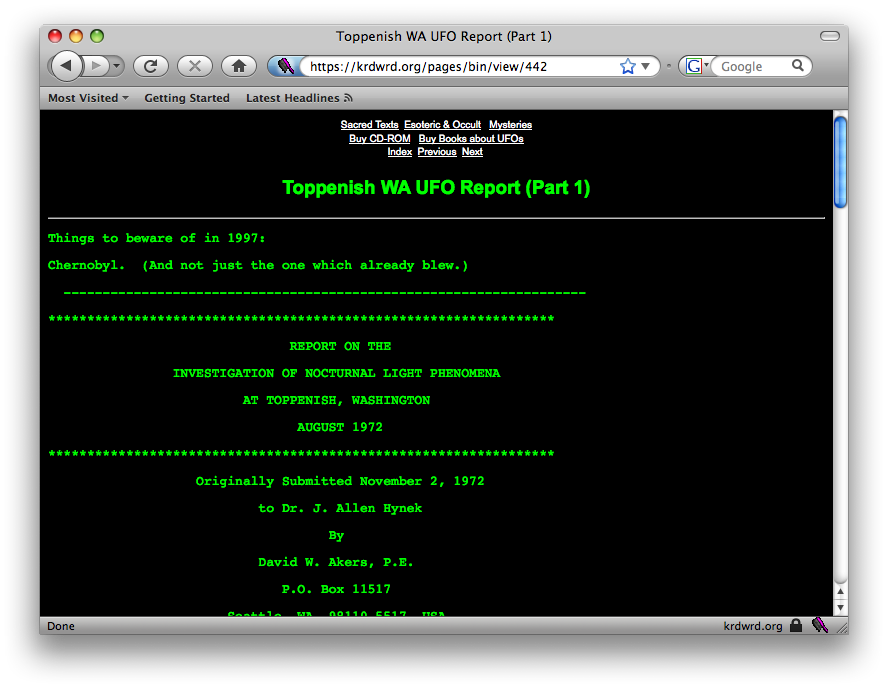
\includegraphics[width=0.6\textwidth]{images/442.png} \\

\end{itemize}
\section{Tips \& Tricks}
\label{TnT}
\subsection{Keyboard Shortcuts}
The default shortcuts for tags are \\
\begin{itemize}
	\item \emph{bad}: ctrl+alt+1
	\item \emph{uncertain}: ctrl+alt+2
	\item \emph{good}: ctrl+alt+3
	\item \emph{clear annotation}: ctrl+alt+4
\end{itemize}

Depending on the size of your keyboard and your hands, this may really hurt after some pages. But you can change the shortcuts. All you need is the \htmladdnormallink{keyconfig}{http://forums.mozillazine.org/viewtopic.php?t=72994} add-on.

\begin{itemize}
	\item \htmladdnormallink{Install keyconfig}{http://mozilla.dorando.at/keyconfig.xpi}.
	\item Bring up the keyconfig menu by pressing \emph{Ctrl+Shift+F12}. (Mac users press \emph{Command+Shift+F12}).
	\item The commands you want to change are named \textbf{Tag Bad}, \textbf{Tag Good} and \textbf{Tag Unknown}.
	\item Close your Firefox window and reopen it; otherwise, the newly set shortcuts will not work.
\end{itemize}


\subsection{How and When To Use Propagate}
\label{TnTProp}
There are two main uses for the propagate utility. Either there are many good text portions embeded in bad text portions (or vice versa). Or there are many small chunks of text cluttered around the page.

With propagate you can often get around tagging each chunk individually.

\begin{itemize}
\item Remember to check each text portion's tag to be correct. \\
\item It is important that text is tagged right, you don't have to care about the background color (and you really shouldn't). \\
\item Propagate will tag text and text only. And you really should not care about the color of the background where the text is written on. \\
\item Most pages in \hyperref{Examples - Medium}{Examples - Medium, page ~}{}{ExMedium} are significantly faster to tag when using the propagate utility. \\
\end{itemize}


\subsection{How to \emph{Undo}}
Currently the add-on has no readily available \emph{Undo} function (which might come handy in cases where you \emph{propagated} the wrong tag). However, the \emph{My~Stats} page lets you \emph{Delete} certain, committed pages. 


\end{document}
